% !TeX root = RJwrapper.tex
\title{ppseq: An R Package for Sequential Predictive Probability
Monitoring}
\author{by Emily C. Zabor, Brian P. Hobbs, and Michael J. Kane}

\maketitle

\abstract{%
Advances in drug discovery have produced numerous biomarker-guided
therapeutic strategies for treating cancer. Yet the promise of precision
medicine comes with the cost of increased complexity. Recent trials of
targeted treatments have included expansion cohorts with sample sizes
far exceeding those in traditional early phase trials of
chemotherapeutic agents. The enlarged sample sizes raise ethical
concerns for patients who enroll in clinical trials, and emphasize the
need for rigorous statistical designs to ensure that trials can stop
early for futility while maintaining traditional control of type I error
and power. The R package \pkg{ppseq} provides a framework for designing
early phase clinical trials of binary endpoints using sequential
futility monitoring based on Bayesian predictive probability. Trial
designs can be compared using interactive plots and selected based on
measures of efficiency or accuracy.
}

\hypertarget{introduction}{%
\section{Introduction}\label{introduction}}

Statistical methods for early phase oncology trials were developed in
the context of cytotoxic treatments. Most cytotoxic treatments exhibit
increases in both efficacy and toxicity with increasing dose. As a
result, phase I trials were centered on identifying the maximum
tolerated dose (MTD), defined as the highest dose that did not exceed a
pre-specified toxicity threshold. Phase I dose-escalation trials were
designed using the rule-based 3+3 method or the model-based continual
reassessment method, among others. But advances in drug discovery have
produced numerous biomarker-guided non-cytotoxic therapies such as small
molecule inhibitors, antibody drug conjugates, immune checkpoint
inhibitors, and monoclonal antibodies. These therapies typically do not
exhibit the same pattern of increases in both efficacy and toxicity with
increasing dose, so the MTD as traditionally defined may not exist.
Instead, lower doses may have equivalent efficacy but lower toxicity as
compared to higher doses. As a result, these therapies can be difficult
to study with traditional dose-escalation designs \citep{Pestana2020}.
To address this issue, recent phase I trials have included large
dose-expansion cohorts, in which additional patients are enrolled in
phase 1 after the dose-escalation phase is complete. In this setup, the
dose-escalation phase is considered phase 1a and used to assess the
initial safety of multiple doses, then the dose-expansion phase is
considered phase 1b and can have a variety of aims including to further
refine the safety of one or more doses, to assess preliminary efficacy,
to explore the treatment in various disease-specific subtypes, or to
further characterize the pharmacokinetics and/or pharmacodynamics. The
use of dose-expansion cohorts increased from 12\% in 2006 to 38\% in
2011 \citep{Manji2013} and trials with dose-expansion cohorts led to
higher response rates and more frequent success in phase 2 trials
\citep{Bugano2017}.

But despite these successes, recent dose-expansion cohorts have not
always been planned in advance, leading to uncertain statistical
properties, and have at times included samples sizes that far exceed
those typically seen in early phase trials of cytotoxic treatments. For
example, the KEYNOTE-001 trial of pembrolizumab, initially designed as a
3+3 dose-escalation trial, included multiple protocol amendments and
ultimately enrolled a total of 655 patients across five melanoma
expansion cohorts and 550 patients across four non-small-cell lung
cancer expansion cohorts \citep{Khoja2015}. In a basket trial of
atezolizumab, an anti-PD-L1 treatment in patients with a variety of
cancers and both with and without PD-L1 expression, an expansion cohort
in metastatic urothelial bladder cancer ultimately enrolled 97 patients
and evaluated 95, despite the fact that no expansion cohort in this
disease subtype was originally planned in the trial protocol. The
expansion cohort in metastatic urothelial carcinoma was rather added
later in a protocol amendment in which the sample size was increased
from what was initially planned \citep{Petrylak2018, Powles2014}. These
enlarged sample sizes raise ethical concerns for patients who enroll in
clinical trials, and emphasize the need for rigorous statistical designs
to ensure that trials can stop early for futility while maintaining
traditional control of type I error and power.

Bayesian predictive probability has been proposed as an approach for
sequential monitoring in early phase oncology trials
\citep{Dmitrienko2006, Lee2008, Hobbs2018, Saville2014}. However, in
order to be useful to investigators designing such trials, software must
be made available to calibrate the design for the desired statistical
properties. To our knowledge no such software currently exists in the R
programming language. This paper introduces the \CRANpkg{ppseq} package
for the R software language \citep{RCT2020}, which provides functions to
design early phase clinical trials of binary endpoints using sequential
predictive probability monitoring for futility. Interactive plots
produced using the \CRANpkg{ggplot2} package \citep{Wickham2016} and the
\CRANpkg{plotly} package \citep{Sievert2020} compare designs based on
different thresholds for decision making. Moreover, we demonstrate
criteria for selecting an ideal predictive probability monitoring design
using the \CRANpkg{ppseq} package. While the \CRANpkg{ppseq} package was
developed with early phase oncology clinical trials in mind, the
methodology is general and can be applied to any application of
sequential futility monitoring in clinical trial design.

\hypertarget{predictive-probability-monitoring}{%
\section{Predictive probability
monitoring}\label{predictive-probability-monitoring}}

Consider the setting of an expansion cohort with a binary outcome, such
as tumor response as measured by the RECIST (Response Evaluation
Criteria in Solid Tumors) criteria. Here we will focus on the one-sample
setting, in which all patients in the trial are enrolled onto a single
arm and given the experimental treatment of interest. Functionality is
also available for the two-sample setting, in which patients are
enrolled onto two different treatment arms, or a treatment and a control
arm, for comparative purposes. Each patient, denoted by \(i\), enrolled
in the trial either has a response such that \(x_i = 1\) or does not
have a response such that \(x_i = 0\). Then \(X = \sum_{i=1}^n x_i\)
represents the number of responses out of \(n\) currently observed
patients up to a maximum of \(N\) total patients. Let \(p\) represent
the true probability of response. Fix \(p_0\) as the threshold for
unacceptable response rate and \(p_1\) as the threshold for acceptable
response rate. Most dose-expansion studies with an efficacy aim will
wish to test the null hypothesis \(H_0: p \leq p_0\) versus the
alternative hypothesis \(H_1: p \geq p_1\).

The Bayesian paradigm of statistics is founded on Bayes' theorem, which
is a mathematical theory that specifies how to combine the prior
distributions that define prior beliefs about parameters, such as the
true response rate \(p\), with the observed data, such as the total
number of responses \(X\), yielding a posterior distribution. Here the
prior distribution of the response rate \(\pi(p)\) has a beta
distribution \(\mbox{Beta}(a_0, b_0)\) and our data \(X\) have a
binomial distribution \(\mbox{Bin}(n, p)\). Combining the likelihood
function for the observed data \(L_x(p) \propto p^x (1-p)^{n-x}\) with
the prior, we obtain the posterior distribution of the response rate,
which follows the beta distribution
\(p|x \sim \mbox{Beta}(a_0 + x, b_0 + n - x)\). A posterior probability
threshold \(\theta\) would be pre-specified during the trial design
stage. At the end of the trial if the posterior probability exceeded the
pre-specified threshold, i.e.~if \(\Pr(p>p_0 | X) > \theta\), the trial
would be declared a success.

The posterior predictive distribution of the number of future responses
\(X^*\) in the remaining \(n^*=N-n\) future patients follows a
beta-binomial distribution
\(\mbox{Beta-binomial}(n^*, a_0 + x, b_0 + n - x)\). Then the posterior
predictive probability (PPP), is calculated as
\(PPP = \sum_{{x^*}=0}^{n^*} \Pr(X^*=x^*|x) \times I(\Pr(p>p_0 | X, X^*=x^*) > \theta)\).
The posterior predictive probability represents the probability that, at
any given interim monitoring point, the treatment will be declared
efficacious at the end of the trial when full enrollment is reached,
conditional on the currently observed data and the specified priors. We
would stop the trial early for futility if the posterior predictive
probability dropped below a pre-specified threshold \(\theta^*\),
i.e.~\(PPP<\theta^*\). Predictive probability thresholds closer to 0
lead to less frequent stopping for futility whereas thresholds near 1
lead to frequent stopping unless there is almost certain probability of
success. Predictive probability provides an intuitive interim monitoring
strategy for clinical trials that tells the investigator what the
chances are of declaring the treatment efficacious at the end of the
trial if we were to continue enrolling to the maximum planned sample
size, based on the data observed in the trial to date.

\hypertarget{package-overview}{%
\section{Package overview}\label{package-overview}}

The \CRANpkg{ppseq} package facilitates the design of clinical trials
utilizing sequential predictive probability monitoring for futility. The
goal is to establish a set of decision rules at the trial planning phase
that would be used for interim monitoring during the course of the
trial. The main computational challenge in designing such a trial is
joint calibration of the posterior probability and posterior predictive
probability thresholds to be used in the trial in order to achieve the
desired levels of frequentist type I error and power. The main function
for achieving this aim is the \texttt{calibrate\_thresholds()} function,
which will evaluate a grid of posterior thresholds \(\theta\) and
predictive thresholds \(\theta^*\) provided by the user as vector inputs
specified with the arguments \texttt{pp\_threshold} and
\texttt{ppp\_threshold}, respectively. Other required arguments include
the unacceptable response rate \(p_0\) specified by \texttt{p\_null},
the acceptable response rate \(p_1\) specified by \texttt{p\_alt}, a
vector of sample sizes at which interim analyses are to be performed
\texttt{n}, and the maximum total sample size \texttt{N}. The direction
of the alternative hypothesis is specified with the argument
\texttt{direction} and defaults to \texttt{"greater"}, which corresponds
to the alternative hypothesis \(H_1: p \geq p_1\). The hyperparameters
of the prior beta distribution are specified with the argument
\texttt{prior} and default to \texttt{c(0.5,\ 0.5)}, which denotes a
\(\mbox{Beta}(0.5, 0.5)\) distribution. The number of posterior samples
are specified with the argument \texttt{S}, which defaults to
\texttt{5000} samples, and the number of simulated trial datasets is
specified with the argument \texttt{nsim}, which defaults to
\texttt{1000}. The additional argument \texttt{delta}, which defaults to
\texttt{NULL} for the one-sample setting, can specify a clinically
meaningful difference between groups \(\delta = p_1 - p_0\) in the case
of a two-sample trial design.

The \texttt{calibrate\_thresholds()} function conducts the following
algorithm, given the default arguments:

\begin{enumerate}
\def\labelenumi{\arabic{enumi}.}
\item
  Generate \texttt{nsim} datasets, denoted by \(j\), containing the
  cumulative number of responses \(x\) at each interim sample size \(n\)
  from a binomial distribution under the unacceptable (i.e.~null)
  response rate \(p_0\), specified by \texttt{p\_null}, and under the
  acceptable (i.e.~alternative) response rate \(p_1\), specified by
  \texttt{p\_alt}, for each interim look, denoted by \(l\).
\item
  For dataset \(j\) and posterior threshold \(\theta_k\), draw
  \texttt{S} samples, denoted by \(s\), from the posterior distribution
  \(p|x_{ls} \sim \mbox{Beta}(a_0 + x_l, b_0 + n_l - x_l)\) where
  \(x_l\) is the number of responses at interim look \(l\) and \(n_l\)
  is the number of enrolled patients at interim look \(l\). Use each
  \(p|x_{ls}\) as the response probability in a binomial distribution to
  generate the number of future responses \(X^*_{ls}\) in the remaining
  \(n^*_l=N-n_l\) future patients at interim look \(l\).

  \begin{enumerate}
  \def\labelenumii{\alph{enumii}.}
  \tightlist
  \item
    Then for each \(X^*_{ls}\), generate \texttt{S} posterior
    probabilities, denoted by \(s'\), at the end of the trial:
    \(PP^*_{lss'} \sim \mbox{Beta}(a_0 + X^*_{ls} + x_l, b_0 + n^*_l - (X^*_{ls} + x_l))\)
    and calculate
    \(PP^*_{ls} = \Pr(p>p_0 | X^*_{ls}) = \frac{\sum_1^{S'} PP^*_{lss'} > p_0}{S'}\).
  \item
    Estimate the predictive probability at posterior threshold \(k\) as
    \(PPP_{lk} = \frac{\sum_1^S PP^*_{ls}>\theta_k}{S}\).
  \item
    Stop the trial for dataset \(j\) at interim look \(l\) and
    predictive threshold \(m\) if \(PPP_{lk} < \theta^*_m\). Otherwise
    continue enrolling.
  \end{enumerate}
\item
  Repeat (2) over all combinations of datasets \(j\), posterior
  thresholds \(k\), and predictive thresholds \(m\).
\item
  If dataset \(j\) was stopped early for futility then we do not reject
  the null hypothesis. If dataset \(j\) reached full enrollment, we
  reject the null hypothesis \(H_0: p \leq p_0\) at posterior threshold
  \(k\) if \(PPP_{lk} > \theta_k\).
\end{enumerate}

The function returns a list, the first element of which is a
\texttt{tibble} containing the posterior threshold \(\theta\), the
predictive threshold \(\theta^*\), the mean sample size under the null
and the alternative, the proportion of positive trials under the null
and alternative, and the proportion of trials stopped early under the
null and alternative. The proportion of trials simulated under the null
hypothesis for which the null hypothesis was rejected is an estimate of
the type I error, and the proportion of trials simulated under the
alternative hypothesis for which the null hypothesis was rejected is an
estimate of the power. The \texttt{print()} option will print the
results summary for each combination of thresholds, filtered by an
acceptable range of type I error and minimum power, if desired. Note
that the results will be sensitive to the choice of \texttt{nsim} and
\texttt{S}. We have set what we believe are reasonable defaults and
would caution users against reducing these values without careful
consideration.

\hypertarget{design-selection}{%
\subsection{Design selection}\label{design-selection}}

After obtaining results for all combinations of evaluated posterior and
predictive thresholds, the next step is to select the ideal design from
among the various options. The \CRANpkg{ppseq} package introduces two
criteria to assist users in making a selection. The first, called the
``optimal accuracy'' design, identifies the design that minimizes the
Euclidean distance to 0 type I error probability and a power of 1. To
accomplish this, the accuracy Euclidean distance (AED) for the design
with posterior threshold \(k\) and predictive threshold \(m\) is
calculated as
\(AED_{km} = w_\alpha * (\alpha_{km} - 0)^2 + w_(1-\beta) * ((1-\beta)_{km}-1)^2\),
where \(w_\alpha\) and \(w_{(1-\beta)}\) are optional weights on the
type I error and power, respectively, and \(\alpha_{km}\) denotes the
estimated type I error and \((1-\beta)_{km}\) denotes the estimated
power. The design with the smallest value of \(AED_{km}\) is selected as
optimal. The second criteria, called the ``optimal efficiency'' design,
identifies the design that minimizes the Euclidean distance to minimal
average sample size under the null and maximal average sample size under
the alternative. To accomplish this, the efficiency Euclidean distant
(EED) for the design with posterior threshold \(k\) and predictive
threshold \(m\) is calculated as
\(EED_{km} = w_{\bar{N}_{H_0}} * (\bar{N}_{H_0km} - min(\bar{N}_{H_0}))^2 + w_{\bar{N}_{H_1}} * (\bar{N}_{H_1km}-max(\bar{N}_{H_1}))^2\),
where \(w_{\bar{N}_{H_0}}\) and \(w_{\bar{N}_{H_1}}\) are optional
weights on the average sample size under the null and alternative,
respectively, \(\bar{N}_{H_0km}\) and \(\bar{N}_{H_1km}\) denote the
average sample sizes under the null and alternative, respectively, and
\(min(\bar{N}_{H_0})\) and \(max(\bar{N}_{H_1})\) denote the minimum
average sample size under the null and the maximum average sample size
under the alternative alternative, respectively, across all combinations
of \(k\) and \(m\). The design with the smallest value of \(EED_{km}\)
is selected as optimal. The \texttt{optimize\_design()} function returns
a list that contains the details of each of the two optimal designs.

\hypertarget{decision-rules}{%
\subsection{Decision rules}\label{decision-rules}}

To ease the implementation of clinical trials designed with sequential
predictive probability monitoring, once a design has been selected, a
table of decision rules can be produced using the
\texttt{calc\_decision\_rules()} function. The function takes the sample
sizes \texttt{n} at which interim analyses are to be performed as well
as the maximum total sample size \texttt{N}, the null value to compare
to in the one-sample case \texttt{p0} (set to \texttt{NULL} in the
two-sample case), the posterior threshold of the selected design
\texttt{theta}, and the predictive threshold of the selected design
\texttt{ppp}. Arguments \texttt{direction}, \texttt{prior}, \texttt{S},
\texttt{delta} are as described in the Package Overview section, with
the same defaults. The function results in a \texttt{tibble}. The trial
would stop at a given look if the number of observed responses is less
than or equal to \(r\), otherwise the trial would continue enrolling if
the number of observed responses is greater than \(r\). At the end of
the trial when the maximum planned sample size is reached, the treatment
would be considered promising if the number of observed responses is
greater than \(r\). In the one-sample case, the resulting
\texttt{tibble} includes a column for the sample size \texttt{n} at each
interim look, \(r\) at each look, and a column for the associated
posterior predictive probability \texttt{ppp}. In the two-sample case,
the \texttt{tibble} includes columns for \texttt{n0} and \texttt{n1},
the sample size at each interim analysis in the control and experimental
arms, respectively. There are also columns for \texttt{r0} and
\texttt{r1}, the number of responses in the control arm and experimental
arm, respectively, leading to the decision to stop or continue. Finally,
there is a column for the posterior predictive probability associated
with that decision \texttt{ppp}.

\hypertarget{visualizations}{%
\subsection{Visualizations}\label{visualizations}}

Finally, to assist users in comparing the results of the various design
options, a \texttt{plot()} option is available for the results of
\texttt{calibrate\_thresholds} that allows creation of static plots
using the \CRANpkg{ggplot2} package \citep{Wickham2016} or interactive
plots using the \CRANpkg{plotly} package \citep{Sievert2020}. Two plots
are produced, one plotting type I error by power and indicating the
optimal accuracy design, and one plotting the average sample size under
the null by the average sample size under the alternative and indicating
the optimal efficiency design. The motivation for including an
interactive graphics option was the utility of the additional
information available when hovering over each point. Instead of simply
eyeballing where points fall along the axes, users can see the specific
type I error, power, average sample size under the null, average sample
size under the alternative, the posterior and predictive thresholds
associated with the design, as well as the distance to the upper left
point on the plot. A \texttt{plot()} option is also available for the
results of \texttt{calc\_decision\_rules}. In the one-sample case it
produces a single plot showing the sample size at each interim analysis
on the x-axis and the possible number of responses at each interim
analysis on the y-axis. In the two-sample case a grid of plots is
produced, with one plot for each interim analysis. The x-axis shows the
number of possible responses in the control group and the y-axis shows
the number of possible responses in the experimental group. In both
cases, the boxes are colored green for a ``proceed'' decision and red
for a ``stop'' decision for each combination and the hover box produced
by \CRANpkg{plotly} provides the details.

\hypertarget{package-demonstration}{%
\section{Package demonstration}\label{package-demonstration}}

In this section I will present a basic example to demonstrate the
functionality included in the \CRANpkg{ppseq}. The following section
will present a more realistic case study.

First we install and load the \CRANpkg{ppseq} package.

\begin{Schunk}
\begin{Sinput}
install.packages("ppseq")
\end{Sinput}
\end{Schunk}

\begin{Schunk}
\begin{Sinput}
library(ppseq)
\end{Sinput}
\end{Schunk}

Consider the case where we are interested in designing a trial to
investigate how a new treatment impacts tumor response measured as a
binary outcome of response versus no response. We know the current
standard of care treatment results in a tumor response rate of 10\%, and
we wish to improve this by 30\%. So we wish to test \(H_0: p \leq 0.1\)
versus \(H_1: p \geq 0.4\), so we set \texttt{p\_null\ =\ 0.1} and
\texttt{p\_alt\ =\ 0.4}. This is a rare disease so our maximum sample
size is 15, so we set \texttt{N\ =\ 15}, and we will do interim analyses
after every 5 patients, so we set \texttt{n\ =\ seq(5,\ 15,\ 5)}. We
wish to examine designs based on combinations of posterior thresholds
\(\theta = {0.85, 0.90}\) and predictive thresholds
\(\theta^*={0.1, 0.2}\), so we set
\texttt{pp\_threshold\ =\ c(0.85,\ 0.9)} and
\texttt{ppp\_threshold\ =\ c(0.1,\ 0.2)}. Finally, for computational
speed in this basic example, we set \texttt{S=50} and \texttt{nsim=50},
but in practice we would want to use much larger values, in the
thousands.

\begin{Schunk}
\begin{Sinput}
set.seed(123)

cal_thresh <-
  calibrate_thresholds(
    p_null = 0.1, 
    p_alt = 0.4,
    n = seq(5, 15, 5), 
    N = 15,
    pp_threshold = c(0.85, 0.9),
    ppp_threshold = c(0.1, 0.2),
    S = 50, 
    nsim = 50
    )
\end{Sinput}
\end{Schunk}

Since there are only four design options in this toy example, we print
the entire results table using a call to \texttt{print()}:

\begin{Schunk}
\begin{Sinput}
print(cal_thresh)
\end{Sinput}
\begin{Soutput}
#> # A tibble: 4 x 8
#>   pp_threshold ppp_threshold mean_n1_null prop_pos_null
#>          <dbl>         <dbl>        <dbl>         <dbl>
#> 1         0.85           0.1         12.1          0.1 
#> 2         0.85           0.2          9.5          0.06
#> 3         0.9            0.1         10.8          0.04
#> 4         0.9            0.2          8.9          0.04
#>   prop_stopped_null mean_n1_alt prop_pos_alt prop_stopped_alt
#>               <dbl>       <dbl>        <dbl>            <dbl>
#> 1              0.42        14.8         0.92             0.02
#> 2              0.64        14.8         0.92             0.02
#> 3              0.5         14.8         0.9              0.02
#> 4              0.74        14.7         0.88             0.04
\end{Soutput}
\end{Schunk}

We use \texttt{optimize\_design()} to identify the optimal accuracy and
optimal efficiency designs, subject to type I error between 0.025 and
0.1, specified by \texttt{type1\_range\ =\ c(0.025,\ 0.1)}, and power of
at least 0.75, specified by \texttt{minimum\_power\ =\ 0.75}:

\begin{Schunk}
\begin{Sinput}
optimize_design(cal_thresh, type1_range = c(0.025, 0.1), minimum_power = 0.75)
\end{Sinput}
\begin{Soutput}
#> $`Optimal accuracy design:`
#> # A tibble: 1 x 6
#>   pp_threshold ppp_threshold `Type I error` Power
#>          <dbl>         <dbl>          <dbl> <dbl>
#> 1         0.85           0.2           0.06  0.92
#>   `Average N under the null` `Average N under the alternative`
#>                        <dbl>                             <dbl>
#> 1                        9.5                              14.8
#> 
#> $`Optimal efficiency design:`
#> # A tibble: 1 x 6
#>   pp_threshold ppp_threshold `Type I error` Power
#>          <dbl>         <dbl>          <dbl> <dbl>
#> 1          0.9           0.2           0.04  0.88
#>   `Average N under the null` `Average N under the alternative`
#>                        <dbl>                             <dbl>
#> 1                        8.9                              14.7
\end{Soutput}
\end{Schunk}

And to ease interim analysis during the course of the trial, we obtain
the decision table using the \texttt{calc\_decision\_rules} function,
with the thresholds of our selected optimal efficiency design passed as
\texttt{theta\ =\ 0.9} and \texttt{ppp\_threshold\ =\ 0.2}. For
computational speed in this basic example, we set \texttt{S=50}, but in
practice we would want to draw many more posterior samples, and values
of 5000 or more should be considered. If any \texttt{NA} value was
returned in this table, it would indicate that at that interim look you
would never stop, regardless of the number of responses.

\begin{Schunk}
\begin{Sinput}
calc_decision_rules(
  n = seq(5, 15, 5), 
  N = 15,
  theta = 0.9,
  ppp = 0.2,
  p0 = 0.1,
  S = 50
)
\end{Sinput}
\begin{Soutput}
#> # A tibble: 3 x 3
#>       n     r   ppp
#>   <dbl> <int> <dbl>
#> 1     5     0  0.06
#> 2    10     1  0.1 
#> 3    15     2  0
\end{Soutput}
\end{Schunk}

This table tells us that at the first interim analysis after we have
observed the first five patients for response, we would stop the trial
if no responses had been observed, and would continue enrolling if at
least one response had been observed. At the second interim analysis
after we have observed the first ten patients for response, we would
stop the trial if zero or one responses had been observed, and would
continue enrolling if at least two responses had been observed. At the
end of the trial after all 15 patients have been observed for response,
we would declare the new treatment promising if at least three responses
had been observed.

\hypertarget{case-study}{%
\section{Case study}\label{case-study}}

The case study focuses on a re-design of a phase II study of
atezolizumab in metastatic urothelial carcinoma patients (mUC) using
sequential predictive probability monitoring. Atezolizumab is a
programmed death-ligand 1 (PD-L1) blocking monoclonal antibody that was
given accelerated approval by the U.S. Food and Drug Administration in
May 2016 for the treatment of patients with locally advanced or
metastatic urothelial carcinoma who had disease progression following
platinum-containing chemotherapy. The approval was based on the results
of a single-arm phase II study in 310 patients \citep{Rosenberg2016}.
The phase II study used a hierarchical fixed-sequence testing procedure
to test increasingly broad subgroups of patients based on PD-L1 status,
and found overall response rates of 26\% (95\% CI: 18-36), 18\% (95\%
CI: 13-24), and 15\% (95\% CI 11-19) in patients with \(\geq5\%\)
PD-L1-positive immune cells (IC2/3 subgroup), in patients with
\(\geq1\%\) PD-L1-positive immune cells (IC1/2/3 subgroup), and in all
patients, respectively \citep{Rosenberg2016}. All three rates exceeded
the historical control rate of 10\%. Then, in March 2021, the approval
in this indication was voluntarily withdrawn by the sponsor following
negative results from a randomized phase III study \citep{Powles2018}.
In the phase III study, 931 patients were randomly assigned to receive
atezolizumab or chemotherapy in a 1:1 ratio, and the same hierarchical
fixed-sequence testing procedure as in the phase II study was used. The
phase III study found that overall survival did not differ significantly
between the atezolizumab and chemotherapy groups of the IC2/3 subgroup
(median survival 11.1 months {[}95\% CI: 8.6-15.5{]} versus 10.6 months
{[}95\% CI: 8.4-12.2{]}), so no further testing was conducted for the
primary endpoint \citep{Powles2018}. Further analyses revealed that
while the response rates to atezolizumab were comparable to those seen
in the phase II study, the response rates to chemotherapy were much
higher than the historical control rate of 10\%. The overall response
rates to chemotherapy were 21.6\% (95\% CI: 14.5-30.2), 14.7\% (95\% CI:
10.9-19.2), and 13.4\% (95\% CI: 10.5-16.9) for the IC2/3 subgroup,
IC1/2/3 subgroup, and all patients, respectively. The overall response
rates to atezolizumab were 23\% (95\% CI: 15.6-31.9), 14.1\% (95\% CI:
10.4-18.5), and 13.4\% (95\% CI: 10.5-16.9) for the IC2/3 subgroup,
IC1/2/3 subgroup, and all patients, respectively. These results indicate
that PD-L1 status is a prognostic biomarker for both standard of care
chemotherapies that comprised the control arm as well as atezolizumab in
this patient population.

We wish to re-design the phase II trial of atezolizumab using a two-arm
randomized design with sequential predictive probability monitoring. We
willuse the \texttt{calibrate\_thresholds()} function to obtain the
operating characteristics of designs based on on each combination of
posterior and predictive thresholds. We focus here on the main biomarker
subgroup of interest, the IC2/3 subgroup. We design the study with a
null response rate of 0.1 in both arms, and an alternative response rate
of 0.25 in the atezolizumab arm. So we set
\texttt{p\_null\ =\ c(0.1,\ 0.1)} and \texttt{p\_alt\ =\ c(0.1,\ 0.25)}.
We plan the study with 100 participants, assuming that the total sample
size available is similar to the 310 used in the actual single-arm phase
II trial, and that a third of that patient population fall into our
desired biomarker subgroup. So we set \texttt{N\ =\ c(50,\ 50)} to
indicate equal allocation of the 100 patients to each of the two arms.
We will check for futility after every 10 patients are enrolled on each
arm, so we set
\texttt{n\ =\ cbind(seq(10,\ 50,\ 10),\ seq(10,\ 50,\ 10))}, a matrix
showing the interim analysis sample sizes in each of the two arms. To
design the study, we need to calibrate the design over a range of
posterior probability thresholds and predictive probability thresholds.
In this example we will consider posterior thresholds of 0.9, 0.91,
0.92, 0.93, 0.94, 0.95, 0.96, 0.97, 0.98, and 0.99, and predictive
thresholds of 0.05, 0.1, 0.15, and 0.2. So we set
\texttt{pp\_threshold\ =\ seq(0.9,\ 0.99,\ 0.01)} and
\texttt{ppp\_threshold\ =\ seq(0.05,\ 0.2,\ 0.05)}. We selected these
posterior thresholds because we want to have a posterior probability of
at least 0.9 that our response rate exceeds the null. And we selected
these predictive thresholds because we would not want to stop the trial
early for futility if there was more than a 20\% chance of success when
full enrollment was reached. We use the defaults for all remaining
arguments, including the defaults of \texttt{S=5000} and
\texttt{nsim=1000}, which we believe are sufficient to obtain stable
results. Because of the inherent computational intensity in these
calculations, this function relies on the \CRANpkg{future}
\citep{Bengtsson2020} and \CRANpkg{furrr} \citep{Vaughan2021} packages
to parallelize computations. The user will be responsible for setting up
a call to \texttt{future::plan()} that is appropriate to their operating
environment and simulation setting. Because the code takes some time to
run, the results of the below example code are available as a dataset
called \texttt{two\_sample\_cal\_tbl} included in the \CRANpkg{ppseq}
package.

\begin{Schunk}
\begin{Sinput}
library(future)

set.seed(123)

future::plan(future::multicore(workers = 40))

two_sample_cal_tbl <- 
  calibrate_thresholds(
    p_null = c(0.1, 0.1), 
    p_alt = c(0.1, 0.25),
    n = cbind(seq(10, 50, 10), seq(10, 50, 10)),
    N = c(50, 50), 
    pp_threshold = seq(0.9, 0.99, 0.01),
    ppp_threshold = seq(0.05, 0.2, 0.05),
    direction = "greater", 
    delta = 0, 
    prior = c(0.5, 0.5), 
    S = 5000, 
    nsim = 1000
  )
\end{Sinput}
\end{Schunk}

We can compare the design options that meet our desired range of type I
error and minimum power by passing the results of our call to the
\texttt{calibrate\_thresholds()} function to the \texttt{plot()}
function. The \texttt{plotly\ =\ TRUE} option produces interactive
visualizations or the \texttt{plotly\ =\ FALSE} option produces static
visualizations.

\begin{Schunk}
\begin{Sinput}
plot(
  two_sample_cal_tbl, 
  type1_range = c(0.05, 0.1), 
  minimum_power = 0.7,
  plotly = TRUE
)
\end{Sinput}
\end{Schunk}

\begin{Schunk}
\begin{figure}
\includegraphics[width=1.1\linewidth]{zabor-hobbs-kane_files/figure-latex/unnamed-chunk-9-1} \caption[Plot of design options made with the {ggplot2} package]{Plot of design options made with the {ggplot2} package. The accuracy designs are on the left and the efficiency designs are on the right. The color represents the Euclidean distance to the top left point and the optimal design is indicated by a diamond.}(\#fig:unnamed-chunk-9)
\end{figure}
\end{Schunk}

We see that the optimal efficiency design is the one with posterior
threshold 0.92 and predictive threshold 0.05. It has a type I error of
0.07, power of 0.7, average sample size under the null of 29 per arm,
and average sample size under the alternative of 46 per arm. This design
would allow us to stop early if the treatment were inefficacious, thus
preserving valuable financial resources for use in studying more
promising treatments and preventing our human subjects from continuing
an ineffective treatment.

\begin{Schunk}
\begin{Sinput}
optimize_design(
  two_sample_cal_tbl, 
  type1_range = c(0.05, 0.1), 
  minimum_power = 0.7
)
\end{Sinput}
\begin{Soutput}
#> $`Optimal accuracy design:`
#> # A tibble: 1 x 6
#>   pp_threshold ppp_threshold `Type I error` Power
#>          <dbl>         <dbl>          <dbl> <dbl>
#> 1         0.86           0.1            0.1 0.751
#>   `Average N under the null` `Average N under the alternative`
#>                        <dbl>                             <dbl>
#> 1                       28.6                              45.1
#> 
#> $`Optimal efficiency design:`
#> # A tibble: 1 x 6
#>   pp_threshold ppp_threshold `Type I error` Power
#>          <dbl>         <dbl>          <dbl> <dbl>
#> 1         0.92          0.05           0.07 0.701
#>   `Average N under the null` `Average N under the alternative`
#>                        <dbl>                             <dbl>
#> 1                       28.6                              45.5
\end{Soutput}
\end{Schunk}

Finally, we generate the decision table associated with the selected
design for use in making decisions at each interim analysis during the
conduct of the trial. Because of the computational time involved, the
results of the below example code are available as a dataset called
\texttt{two\_sample\_decision\_tbl} included in the \CRANpkg{ppseq}
package. In the results table, we see that at the first interim futility
look after just 5 patients, we would not stop the trial. After the first
10 patients we would stop the trial if there were 0 responses, and so
on. At the end of the trial when all 95 patients have accrued, we would
declare the treatment promising of further study if there were greater
than or equal to 14 responses.

\begin{Schunk}
\begin{Sinput}
set.seed(123)

two_sample_decision_tbl <- 
  calc_decision_rules(
    n = cbind(seq(10, 50, 10), seq(10, 50, 10)),
    N = c(50, 50),
    theta = 0.92, 
    ppp = 0.05, 
    p0 = NULL, 
    direction = "greater", 
    delta = 0, 
    prior = c(0.5, 0.5), 
    S = 5000
    )
\end{Sinput}
\end{Schunk}

The resulting table contains all possible combinations of responses in
the two arms, so is quite long. We can visualize the resulting decision
rules by passing the results of the call to the
\texttt{calc\_decision\_rules()} function to the \texttt{plot()}
function, which returns a faceted plot according to the interim look.
The color denotes whether the trial should proceed (green) or stop (red)
for a given combination of number of responses in the control arm
(x-axis) and number of responses on the experimental arm (y-axis). For
example, we see that at the second interim look when there are 20
patients enrolled on each arm, if there were 10 responses in the control
arm, we would stop the trial if there were 8 or fewer responses on the
experimental arm; otherwise we would proceed with enrollment.

\begin{Schunk}
\begin{Sinput}
plot(two_sample_decision_tbl, plotly = FALSE)
\end{Sinput}
\begin{figure}
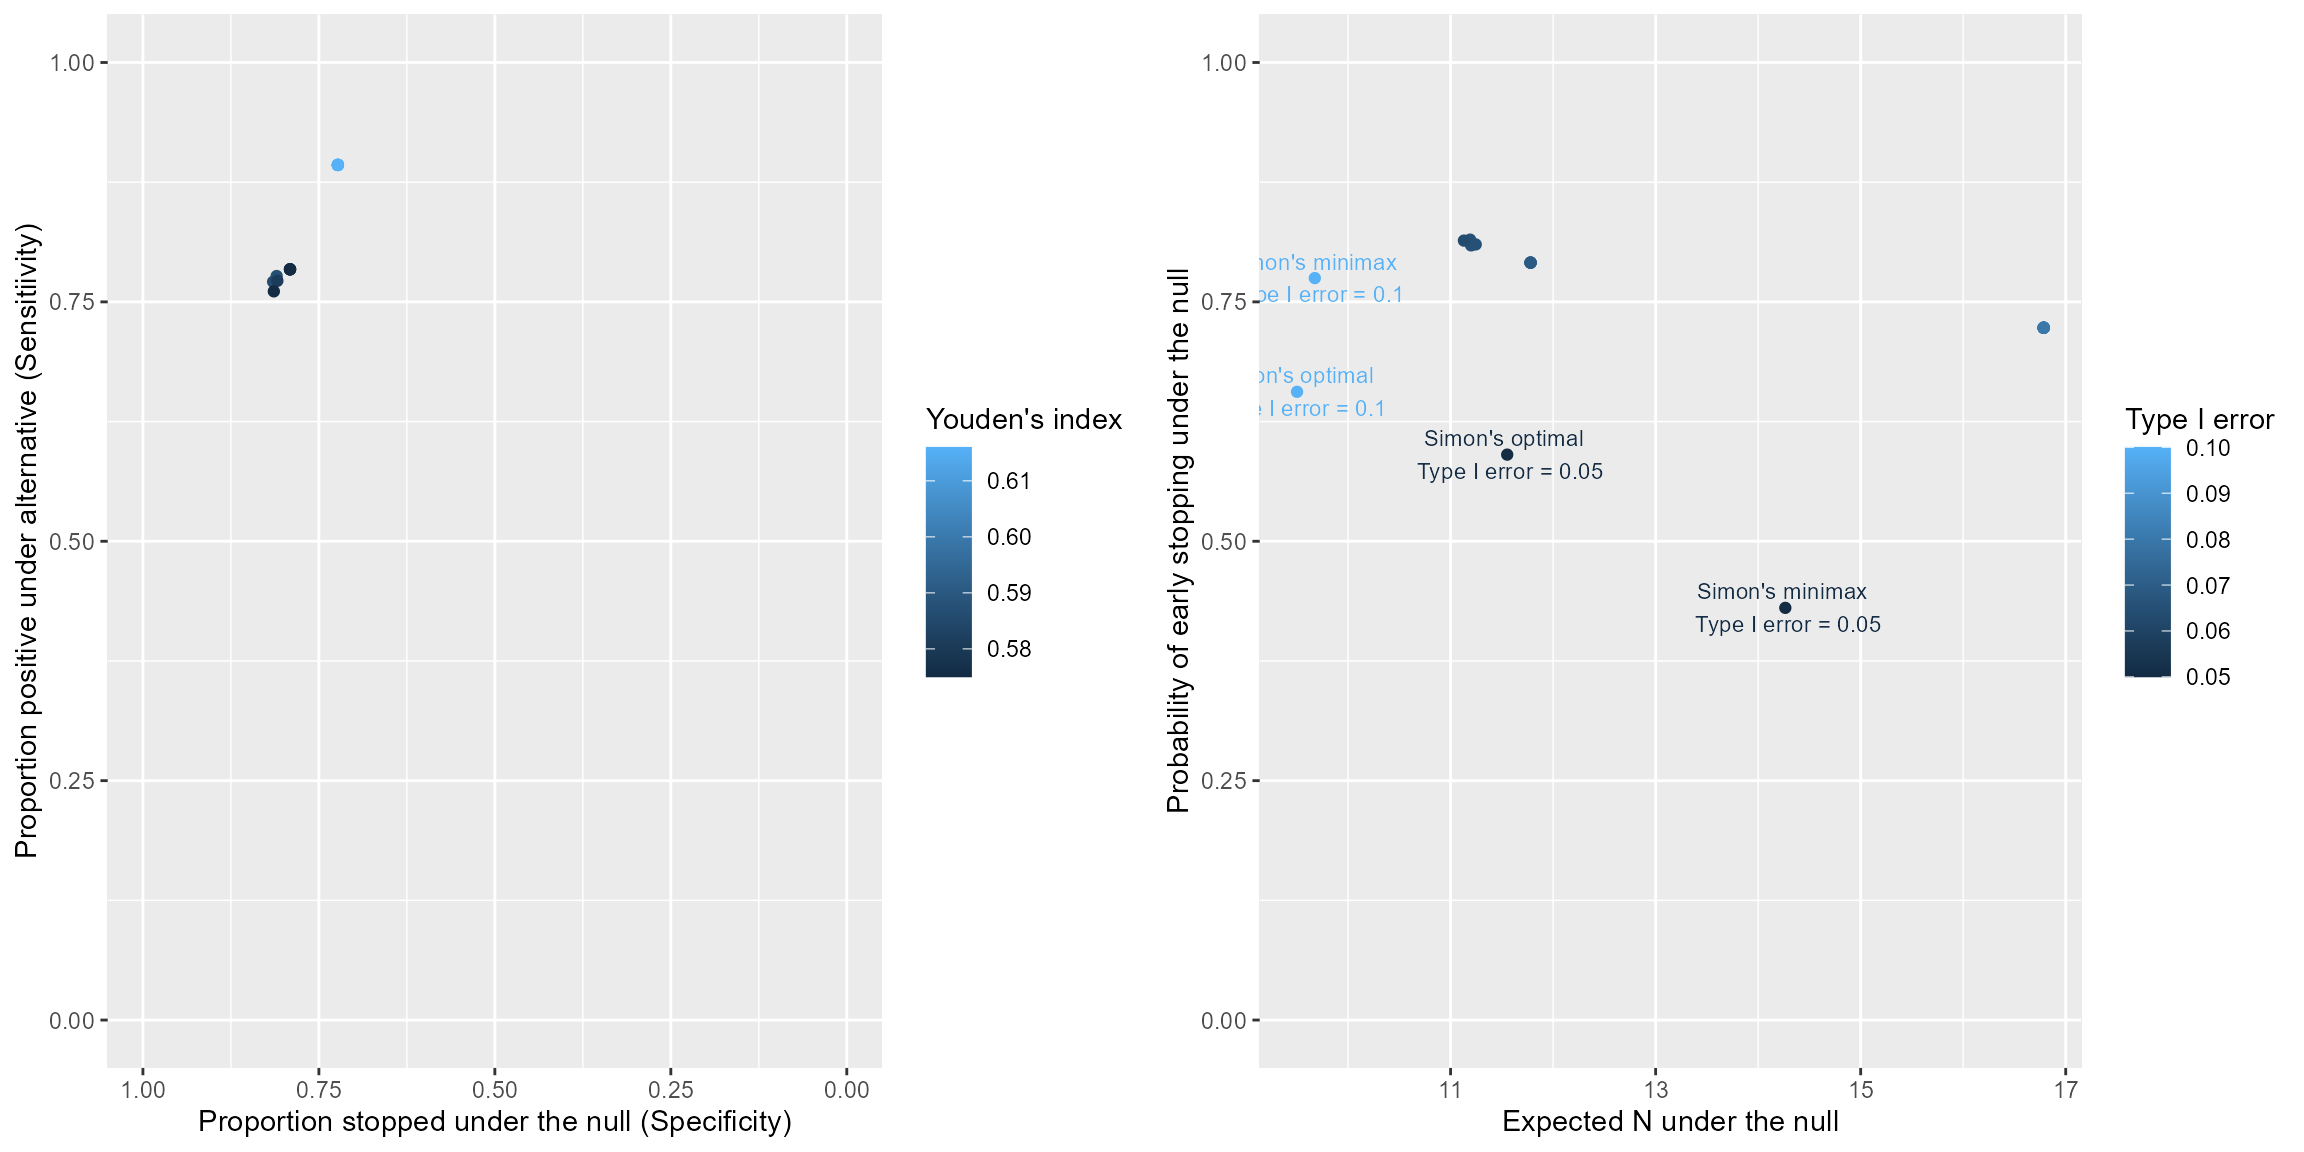
\includegraphics{zabor-hobbs-kane_files/figure-latex/unnamed-chunk-13-1} \caption[Plot of decision rules made with ggplot]{Plot of decision rules made with ggplot. The color indicates whether the trial should stop or proceed for a given number of responses at each interim analysis.}(\#fig:unnamed-chunk-13)
\end{figure}
\end{Schunk}

\hypertarget{summary}{%
\section{Summary}\label{summary}}

With the focus of early stage clinical trial research in oncology
shifting away from the study of cytotoxic treatments and toward
immunotherapies and other non-cytotoxic treatments, new approaches to
clinical trial design are needed that move beyond the traditional search
for the maximum tolerated dose \citep{Hobbs2019}. Bayesian sequential
predictive probability monitoring provides a natural and flexible way to
expand the number of patients studied in phase 1 or to design phase 2
trials that allow for efficient early stopping for futility while
maintaining control of type I error and power. The \CRANpkg{ppseq}
package implements functionality to evaluate a range of posterior and
predictive thresholds for a given study design and identify the optimal
design based on accuracy (i.e.~type I error and power) or efficiency
(i.e.~average sample sizes under the null and alternative). Interactive
visualization options are provided to ease comparison of the resulting
design options. Once an ideal design is selected, a table of decision
rules can be obtained to make trial conduct simple and straightforward.

\begin{verbatim}
\end{verbatim}

\bibliography{zabor-hobbs-kane.bib}

\address{%
Emily C. Zabor\\
Department of Quantitative Health Sciences \& Taussig Cancer Institute,
Cleveland Clinic\\%
9500 Euclid Ave. CA-60\\ Cleveland, OH 44195 USA\\
%
\url{http://www.emilyzabor.com/}\\%
\textit{ORCiD: \href{https://orcid.org/0000-0002-1402-4498}{0000-0002-1402-4498}}\\%
\href{mailto:zabore2@ccf.org}{\nolinkurl{zabore2@ccf.org}}%
}

\address{%
Brian P. Hobbs\\
Dell Medical School, The University of Texas at Austin\\%
true\\ Austin, TX 78712\\
%
%
\textit{ORCiD: \href{https://orcid.org/0000-0003-2189-5846}{0000-0003-2189-5846}}\\%
\href{mailto:brian.hobbs@austin.utexas.edu}{\nolinkurl{brian.hobbs@austin.utexas.edu}}%
}

\address{%
Michael J. Kane\\
Department of Biostatistics, Yale University\\%
60 College Street\\ New Haven, CT 06511\\
%
%
\textit{ORCiD: \href{https://orcid.org/0000-0003-1899-6662}{0000-0003-1899-6662}}\\%
\href{mailto:michael.kane@yale.edu}{\nolinkurl{michael.kane@yale.edu}}%
}
